\chapter{Primera aproximación a una métrica apropiada. Distancia de Levenshtein}
\label{ch:Levenshtein}

\lettrine[lraise=-0.1, lines=2, loversize=0.2]{L}{a} distancia de Levenshtein
recibe su nombre del científico ruso Vladimir Levenshtein, quién la creó en 1965.

% Definir la distancia de Levenshtein original (citarlo bien)
\vspace{0.3cm}
\textit{"La distancia de Levenshtein, distancia de edición o distancia entre
palabras es el número mínimo de operaciones requeridas para transformar una cadena
de caracteres en otra"}.
\vspace{-0.2cm}
{\flushleft{\hfill \emph{- Wikipedia, 2020, párrafo 1,} \cite{Wikipedia}}}
\vspace{0.3cm}

% Explicar la modificación realizada para adaptarlo a nuestro caso
Aunque este algoritmo esté concebido como métrica de la diferencia entre dos
cadenas de caracteres, podemos aplicar el concepto básico a dos salidas de la
campaña de inyección de fallos. Redefiniendo la distancia de Levenshtein para
nuestro caso en particular:

\vspace{0.3cm}
\textit{"La distancia de Levenshtein es el número mínimo de bits que hay que
conmutar de la salida de una campaña de inyección de fallos para transformarla 
en otra"}.
\vspace{0.3cm}

Existe una operación lógica ya mencionada anteriormente que permite comparar dos
salidas obteniendo como resultado ceros para aquellos bits en los que son iguales
y unos en los diferentes. La operación \textit{XOR} bit a bit permite obtener
tantos unos como diferencias existen entre las dos salidas. La distancia de
Levenshtein entre dos salidas de una campaña es el sumatorio de todos estos bits 
con valor lógico alto.

% Comentar la hipótesis realizada para diagnosticar en base a esto
    % Si el SEU se encuentra en el diccionario -> levenDist = 0
    % Si el SEU no se encuentra en el diccionario -> min(levenDist) será el más
    % cercano
De esta forma, según la hipótesis inicial \ref{hyp:inicial}, dos \gls{SEU}
que estén próximos entre sí tendrán una distancia de Levenshtein relativamente
baja entre ellos. Cuando el diccionario de fallos contiene el error lógico a
diagnosticar, existirá al menos una entrada con la cual la distancia de
Levenshtein será cero. Cuando esto sucede, damos al diagnóstico por terminado,
aunque en el capítulo \ref{ch:CampanasIterativas} veremos una ampliación de la 
técnica que permite continuar un poco más y aumentar la confianza en los 
resultados obtenidos. En caso contrario, las entradas a menor distancia del run a
diagnosticar (de aquí en adelante \textit{"target run"}) serán utilizadas para
localizarlo.


\section{Elaboración de la base de datos de distancias}
\label{sec:LevenDist}
% Explicar como se calculan las distancias de Leven y como se almacenan en memoria
Antes de explicar más concretamente cómo se calculan las distancias entre runs del
diccionario y se elabora la tabla de distancias, es necesario comentar cómo está
expresada inicialmente la información de las salidas una vez son comparadas con el
\textit{Golden run} (ver figura \ref{fig:PostprocesadoSalida}). Un detalle hasta 
ahora no mencionado es que el diccionario se divide en dos archivos,
\textit{"damages.csv"} e \textit{"injections.csv"}. Cada run divide su información
entre estos dos ficheros, ubicando ciclo y \gls{FF} de la inyección en 
\textit{injections.csv} y los errores que esta genera a la salida del circuito, en
\textit{"damages.csv"}.
Para explicar como está dispuesta la información dentro de este último documento 
vamos a suponer que el \gls{CUT} tiene 8 salidas y cada ejecución de la campaña 
dura 10 ciclos de reloj. Un ejemplo de salida contenida en el diccionario de este
circuito puede ser:

\begin{center}
    0:1A,3:C0,4:80,7:1E,8:1C,9:02
\end{center}

% Hex -> binario almacenado como enteros -> XOR bit a bit -> sumatorio de 1s
Cada pareja de números separados por dos puntos significan
\textit{"Ciclo:Fallos"}, donde \textit{Fallos} es una representación hexadecimal
de las salidas del \gls{CUT} en el ciclo \textit{Ciclo}. Los fallos de distintos 
ciclos están separados entre sí mediante comas, y cada run contenido en el 
diccionario se encuentra en una línea independiente. Podemos observar en el 
ejemplo anterior que ciertos ciclos no aparecen. Estos son los ciclos de la 
ejecución donde la salida no presenta discrepancias con el \textit{Golden run}. 
De esta forma, las inyecciones que no generen fallos a la salida del circuito se 
corresponderán con líneas vacías del diccionario.

Ahora que conocemos cómo está contenida la información en el diccionario de
fallos, podemos proceder al cálculo de las distancias. El primer paso es leer la
información de ambos archivos y cargarlos en memoria, rellenando los ciclos sin
fallos con ceros. Hemos decidido almacenar la información en forma de enteros 
en base 10, aunque estos sean tratados como binario. A continuación se realiza, bit
a bit, la \textit{XOR} de cada run con el resto. Como último paso en el cálculo de
las distancias de Levenshtein, se toman los resultados de la operación lógica y se
suman los bits con valor lógico alto. El resultado de esta suma es la distancia
en cuestión.

% Imagen 1: De HEX a binario -> XOR con otro run -> sumatorio -> distancia
\begin{figure}[htbp]
    \centering
    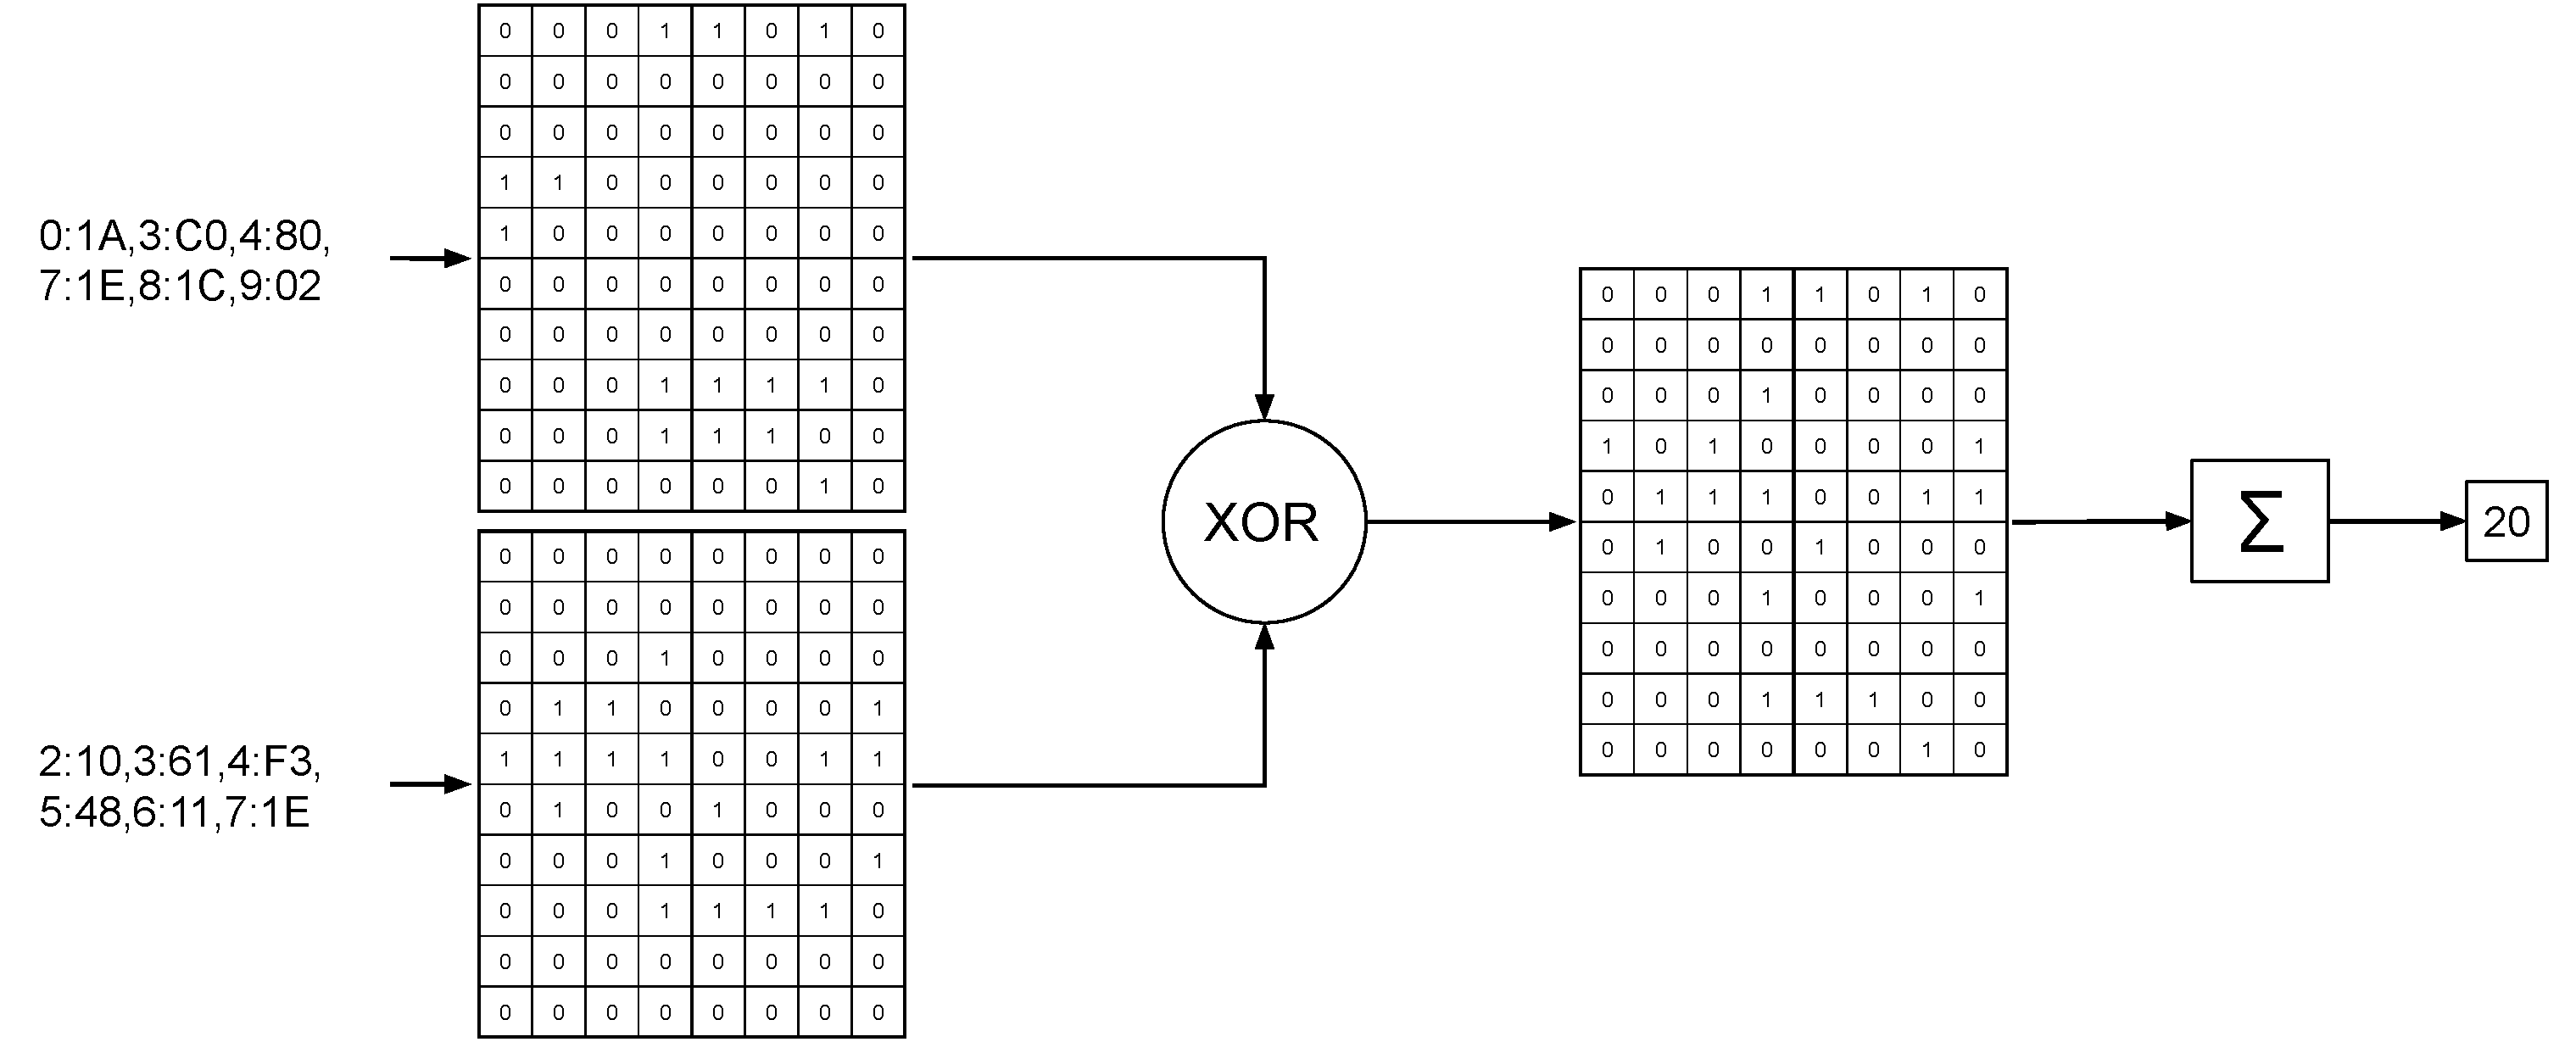
\includegraphics[width=0.95\linewidth]
    {Levenshtein/figuras/fig41.pdf}
    \caption{Cálculo de la distancia de Levenshtein}
    \label{fig:LevenDist}
\end{figure}

% Esto para cada entrada del diccionario -> se obtiene tabla simetrica de
% distancias respecto a la diagonal.
Podemos elaborar una lista con las distancias entre el \textit{target run} y 
todas las entradas del diccionario de forma que la componente \textit{"i"} sea 
la distancia de Levenshtein entre el \gls{SEU} a diagnosticar y la entrada 
\textit{"i"}. Acompañando a esta lista tendríamos otra en la que se encuentra la
información de las inyecciones. 

Por último, notar que al tratarse de distancias, se cumplen las propiedades
típicas de una distancia: 
\begin{center}
    \textit{D(i,i) == 0}

    \textit{D(i,j) == D(j,i)}
\end{center}

\section{Diagnóstico basado en la distancia de Levenshtein}
\label{sec:LevenCands}
% Explicar cómo se seleccionan los candidatos en base a las distancias calculadas
% y por qué se selecciona de esa manera y no de otra. En one note hay apuntes de
% esto
Una vez hayamos calculado las distancias de Levenshtein entre el \textit{target
run} y todas las entradas del diccionario y hayamos elaborado las dos listas
mencionadas tendremos todo lo necesario para llevar a cabo el diagnóstico con esta
primera versión de la técnica. 

Tal y como hemos explicado en el último párrafo del apartado \ref{ch:Levenshtein},
las entradas del diccionario cuyas inyecciones se encuentren más próximas a la
que habría provocado al \textit{target run} presentarán las menores distancias
hasta el mismo. Diagnosticar consiste en seleccionar estas entradas, las cuales
pasarán a llamarse \textit{"Candidatos"}.

Originalmente, el proceso que seguíamos para seleccionar candidatos consistía en
establecer una distancia de corte en función de las distancias máxima y mínima. El
corte se establecía según el porcentaje especificado del rango sobre el mínimo. De
esta forma, eran seleccionados todos runs cuya distancia era menor o igual que el
valor establecido:
% Ecuacion del porcentaje
\begin{equation}
    \label{eq:SeleccionPorcentaje}
    D(i) \leq tolerancia \times \frac{(max - min)}{100} + min
\end{equation}
Donde tolerancia establecía qué porcentaje del rango de distancias se toma. De 
esta forma, todos aquellos runs cuyas distancias cumplían la ecuación
\ref{eq:SeleccionPorcentaje} pasaban a ser candidatos.

% Problemas detectados con este sistema de selección.
El problema de este sistema es que no controlábamos cuántos candidatos
seleccionábamos en cada ocasión. Para valores de tolerancia de 1 a 5, se obtenían
cantidades de candidatos bastante dispares en los diseños de circuitos en que se
probó. Los causantes son valores de distancias aislados y alejados del resto, es
decir, un mínimo o un máximo aislado mucho menor o mayor que el resto
respectivamente. Esto provoca que el rango de distancias se alargue y se
concentren todas muy próximas al extremo, seleccionando bien muy pocos o bien
demasiados candidatos respectivamente.

% La version final... ordenar y coger los n primeros
Este problema puede solucionarse si se identifican y descartan estas distancias
antes de calcular el valor de corte, pero si analizamos bien, veremos que hay una 
solución mejor: ordenar la lista de distancias de menor a mayor y seleccionar las 
entradas correspondientes a las \textit{"n"} primeras distancias, siendo 
\textit{"n"} el número de candidatos que deseemos seleccionar, especificado como 
argumento de entrada.

\section{Resultados experimentales}
\label{sec:LevenResults}
Aunque se realizaron bastantes experimentos hasta llegar a la solución última de
seleccionar los \textit{"n"} primeros runs, hablaremos solo de aquellos resultados
correspondientes a la versión última de este algoritmo.

Para probar la técnica disponíamos de una serie de circuitos con sus respectivos
diccionarios de fallos. Algunos de estos eran exhaustivos, mientras que de otros,
debido al tamaño del circuito, solo disponíamos de uno incompleto fruto de una
campaña de inyección de fallos aleatoria. Concretamente disponíamos de un
diccionario del 0'005\% de exhaustividad para el diseño de la \textit{FFT}, 0'87\%
para la \textit{UART} y 37'78\% para el \textit{FIR\_RI}.

En total, hemos probado el algoritmo en 10 diseños distintos:
\begin{itemize}
    \item Sumador (\textit{adder\_acum}): suma de forma acumulativa los 8 bits de 
        entrada en un registro de 20 bits.
    \item Contador (\textit{counter}): contador de 8 bits.
    \item Doble contador (\textit{dual\_counter}): dos contadores de 8 bits
        conectados formando uno de 16 bits.
    %\item FFT (\textit{fft}): implementa la transformada rápida de Fourier
    %    (\gls{FFT}) \cite{FFT}.
    \item FIFO (\textit{fifo}): memoria de 32 bits del tipo "Primero que entra,
        Primero que sale" (\gls{FIFO}) \cite{FIFO}.
    \item Filtro de respuesta de impulso finito (\textit{FIR\_RI}) \cite{FIR}
    \item PCM (\textit{pcm}): implementa una interfaz I²C para el códec PCM3168
        \cite{PCM}
    \item Registro de desplazamiento (\textit{shiftreg}): registro de
        desplazamiento de 8 bits.
    \item Maquina de estados finita (\textit{simple\_fsm}): maquina de estados
        (\gls{FSM}) con 4 estados.
    \item UART (\textit{uart}): Transmisor y receptor asíncrono universal
        (\gls{UART}), dispositivo para comunicaciones serie \cite{UART}
\end{itemize}

\subsection{Diccionarios exhaustivos}
\label{subsec:LevDicExhaust}
% Siempre aparece mínimo el correcto, a veces más debido a colisiones
Con el uso de diccionarios completos para el diagnóstico se obtiene siempre al 
menos un candidato con el que los patrones de error a la salida coinciden al
completo, ya que todas las combinaciones posibles de \textit{(\gls{FF}, ciclo)}
han sido inyectadas, y por tanto, el target run también.

Como el algoritmo de selección obtiene \textit{"n"} candidatos, también es posible
que obtengamos candidatos a distancia mayor que cero. Como el algoritmo nos
muestra a la salida la distancia de Levenshtein que tiene cada candidato al target
run, podemos descartar manualmente los candidatos que no estén a distancia cero
cuando existan otros que si lo estén como es el caso.

En algunos circuitos obtenemos de hecho varios candidatos a distancia nula. Esto
es debido a colisiones, y es indistinguible de cuál de ellas se trata el target
run realmente.

\subsection{Diccionarios no exhaustivos}
\label{subsec:LevDicNoExhaust}
Para simular diccionarios no exhaustivos en todos los circuitos, realizamos un
pequeño script que eliminaba aleatoriamente entradas del diccionario con una
probabilidad concreta en función del porcentaje de exhaustividad que deseásemos.
La mayor parte de los experimentos se ha realizado con diccionarios del 5\% de
exhaustividad, siendo inferior en aquellos diccionarios que ya lo eran.

Para diccionarios originalmente exhaustivos, seleccionamos aleatoriamente 100
entradas del diccionario original a modo de objetivos a diagnosticar. Como el
nuevo diccionario reducido es también aleatorio, podían estar contenidos o no en
el diccionario. Por el contrario, en diccionarios ya muy incompletos, el
procedimiento que seguimos fue extraer 100 targets del diccionario original,
obteniendo uno nuevo con 100 entradas menos. Para estos circuitos, el target run
no se encontraba en el diccionario.

% Tabla de resultados solo con leven. 5 cands, 5% o menos, reg
\begin{table}[htbp]
    \ttabbox
    {\caption{Resultados experimentales. Distancia de Levenshtein. Dic.
    incompletos ($\leq5\%$)}
    \label{tab:LevenRes}}
    {
        \begin{tabular}{c|c c}
            \hline
            \rule[-8pt]{0pt}{22pt}{\bfseries{Diseños}}&{\bfseries{Registro}}
            &{\bfseries{\gls{FF}}} \\
            \hline
            \rule{0pt}{14pt}adder\_acum & 100 & 98\\
            counter & 100 & 96\\
            dual\_counter & 99 & 99\\
            fifo & 98 & 1\\
            fir\_ri (37'78\%) & 29 & 3\\
            pcm & 82 & 69\\
            shiftreg & 100 & 82\\
            simple\_fsm & 100 & 88\\
            uart (0'87\%) & 97 & 93\\
            \hline
        \end{tabular}
    }
\end{table}

% Explicar el contenido de la tabla: registros correctos de cada 100, FF correctos
% de cada 100, y que se considera registro y FF
En la tabla \ref{tab:LevenRes} se muestran los resultados de las 100 simulaciones
para cada circuito. La columna \textit{Registro} indica cuántas de las 100 veces
se encontraba el registro correcto entre los \textit{"n"} candidatos
seleccionados, en este caso 5 candidatos. Análogamente, la columna
\textit{\gls{FF}} es cuántas de las 100 veces se encontraba el FF correcto entre
los candidatos. Cuando entre los 5 candidatos de una ejecución estaban más de una
vez, se contaba como uno solo para el total de las 100 ejecuciones. La tabla es
una medida de la efectividad de esta distancia como método de diagnóstico aislado
(aunque no se ha tenido en cuenta el ciclo de inyección para realizar el recuento
de aciertos).

Cabe mencionar que \textit{\gls{FF}} es el biestable de inyección y 
\textit{Registro} el resto de la dirección de inyección en caso de existir. En el
caso del \textit{simple\_fsm}, no existen registros, y tanto \textit{adder\_acum}
como \textit{counter} y \textit{shiftreg} tienen un único registro. El 100\% de 
aciertos en estos tres casos no es significativo.

% Decir que se observaba relacion entre distancia de levenshtein y los ciclos o FF
% de inyeccion. Cuando estos aumentaban, la primera lo hacía en sintonía, por eso
% se decidió implementar la distancia en ciclo
Observando los candidatos que seleccionaba el algoritmo y comparando sus
distancias de Levenshtein y la información de sus inyecciones con la inyección 
del target run, la cual conocíamos (por supuesto el algoritmo no tenía acceso a 
ella) se observaba relación directa entre la diferencia de los ciclos de las
inyecciones y la distancia de Levenshtein. Mostrando un número mayor de candidatos
pudimos comprobar como efectivamente, cuando la distancia de Levenshtein
aumentaba o disminuía, también lo hacía la diferencia entre los ciclos de 
inyección. Tras esta observación decidimos implementar una nueva métrica con el
objetivo de mejorar los resultados del diagnóstico.

\endinput
